\documentclass{article}[12pt]

\usepackage{graphicx}
\usepackage[slovene]{babel}
\usepackage{psfrag}
\usepackage{epsf}
\usepackage{amsmath,amsfonts,amssymb,latexsym}
\usepackage{enumitem}
\usepackage[width=175mm,height=260mm,left=20mm,foot=10mm]{geometry}
\usepackage[utf8]{inputenc}
\usepackage{setspace}
\usepackage{epstopdf}
\usepackage[framed,numbered,autolinebreaks,useliterate]{mcode}
\usepackage{float}
%\doublespacing


\newtheorem{izrek}{Izrek}
\newtheorem{posledica}[izrek]{Posledica}
\newtheorem{lema}[izrek]{Lema}
\newtheorem{trditev}[izrek]{Trditev}
\newtheorem{domneva}[izrek]{Domneva}
\newtheorem{problem}[izrek]{Problem}
\newtheorem{vprasanje}[izrek]{Vprasanje}
\newtheorem{definicija}[izrek]{Definicija}
\newtheorem{opomba}[izrek]{Opomba}


\title{Matematična Fizika 1, domača naloga:\\
Preizkus generatorja slučajnih števil porazdeljenih po Poissonovi porazdelitvi}

     \author{
     \textsc{Rok Mihevc} \\[0.25em]
     {\small{Fakulteta za matematiko in fiziko}} \\[-0.25em]
     {\small{Univerza v Ljubljani}} \\[-0.25em]
     {\small\texttt{rok@mihevc.org}}
     }

\date{\today}



%%%%%%%%%%%%%%%%%%%%%%%%%%%%%%%%%%%%%%%%%%%%%%%%%%%%%%%%
%
% Author's definitions


\newenvironment{dokaz}%
{\noindent{\bf Dokaz.}\ }%
{\hfill$\Box$\par\bigskip}%

%%%%%%%%%%%%%%%%%%%%%%%%%%%%%%%
% mno?ice in funkcije
%%%%%%%%%%%%%%%%%%%%%%%%%%%%%%%
\newcommand{\dfnc}[3]{#1:#2\rightarrow #3}
\newcommand{\dset}[2]{\left\{#1 \:|\: #2\right\}}
\newcommand{\lset}[2]{\left\{#1, \ldots, #2\right\}}

%%%%%%%%%%%%%%%%%%%%%%%%%%%%%%%
% ?tevilske mno?ice
%%%%%%%%%%%%%%%%%%%%%%%%%%%%%%%

\newcommand{\NN}{\mathbb N}
\newcommand{\ZZ}{\mathbb Z}
\newcommand{\QQ}{\mathbb Q}
\newcommand{\RR}{\mathbb R}

%%%%%%%%%%%%%%%%%%%%%%%%%%%%%%%
% posebne prilagoditve ukazov
%%%%%%%%%%%%%%%%%%%%%%%%%%%%%%%
\newcommand{\cali}[1]{{\cal #1}}
\def\thx{\vartheta}
\def\epx{\varepsilon}
\def\rhx{\varrho}
\def\phx{\varphi}

\newcommand{\textem}[1]{{\sl #1}}

\renewcommand\a{\alpha}
\renewcommand\b{\beta}
\renewcommand\d{\delta}
\newcommand\D{\Delta}

\begin{document}

\maketitle


\section{Uvod}

Za preskus generatorjev slučajnih števil uporabljajo tudi takoimenovani »run-up« test: v danem vzorcu števil preštejemo, koliko je v njem striktno naraščajočih (padajočih) nizov z dolžino M. Izračunamo pričakovane vrednosti števila nizov z dolzino 1, 2, 3, ..., v naključnem vzorcu 1 milijon števil, porazdeljenih po Poissonovi porazdelitvi. (Slika \ref{plot1})

\begin{figure}[h]
\begin{center}
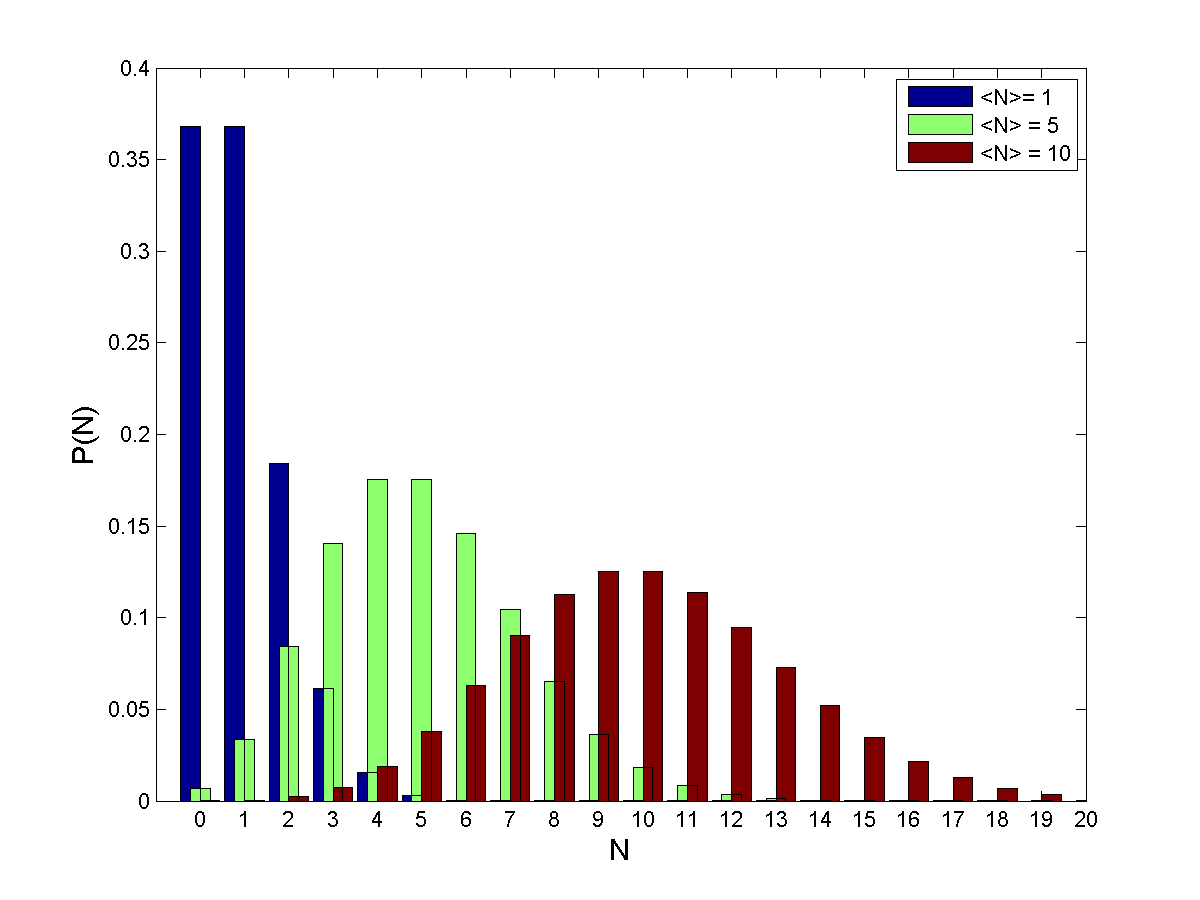
\includegraphics[width=17cm]{slike/plot1}
\caption{Poissonova porazdelitev}
\label{plot1}
\end{center}
\end{figure}

\section{Analitični izračun}

\subsection{Poissonova porazdelitev}

Poissonova porazdelitev je diskretna verjetnostna porazdelitev, ki nam poda \textit{verjetnost danega števila dogodkov N, v danem prostorskem ali časovnem intervalu, pri znani pogostosti teh dogodkov $\bar{N}$}.\\
Izpeljemo jo iz binomske verjetnostne porazdelitve kot njen limitni primer.\\
\[ 
P(N) = e^{-\bar{N}} \cdot \frac{\bar{N}^N}{N!}
\]
Kumulativno verjetnost pa zapišemo kot:

\[ 
F(N) = e^{-\bar{N}} \cdot \sum_{i=0}^{N} \frac{\bar{N}^i}{i!}
\]

Za potrebe te naloge se bomo zaradi preprostosti omejili na primer $\bar{N}=1$.

\subsection{Verjetnost monotono naraščajočega zaporedja}

Odločimo se da bom preučili nize števil, ki strogo naraščajo ($N_2 > N_1$).
Ko iz poissonove naključne porazdelitve zajamamemo vrednost $N_1$, je verjetnost, da smo izbrali $N_1$ in da bo naslednje poissonovo naključno zajeto število $N_2$ večje enaka:
\[
P(N_2 > N_1) = P(N_1) \sum_{N_2=N_1+1}^{\inf} P(N_2) = P(N_1) \cdot (1 - F(N_1))
\]
Zaradi praktičnosti uvedemo notacijo:\\
$P_+(M) = P(N_1 < N_2 < \cdots < N_{M-1} < N_M)$ - verjetnost za strogo naraščujoč niz dolžine M\\
$P_-(M) = P(N_1 > N_2 > \cdots > N_{M-1} > N_M)$ - verjetnost za strogo padajoč niz dolžine M\\
$P_=(M) = P(N_1 = N_2 = \cdots = N_{M-1} = N_M)$ - verjetnost za niz enakih vrednosti N dolžine M\\
$P_+$ - verjetnost za verjetnost za strogo naraščujoč niz\\
$P(M)$ - verjetnost za niz dolžine M\\
$N_+(M) = N(N_1 < N_2 < \cdots < N_{M-1} < N_M)$ - število strogo naraščujočih nizov dolžine M\\
$N_-, N_=, P_-,P_=$ - analogno\\

Prejšen izraz posplošimo na vse možne $N_i$ in vse možne nize števil $N_1<N_2<\cdots<N_{M-1}<N_M$ pri dolžini niza M dobimo rahlo nepregledno formulo:
\[
P_+(M) = \sum_{N_1=0}^{\inf} \left( P(N_1) \sum_{N_2=N_1+1}^{\inf} \left( P(N_2) \cdots \sum_{N_{M-1}=N_{M-2}+1}^{\inf} \left( P(N_{M-1})(1 - F(N_{M-1}) \right)\right)\right)
\] 
Za reševanje te enačbe se zdi primerno orodje rekurzivna funkcija:
\lstinputlisting{../octave/zap.m}

Možno pa je tudi reševanje z matriko kombinacij - zapišemo matriko vseh možnih zaporedij, kjer so vrstice možna zaporedja. Nato izračunamo verjetnosti za te elemente in jih zapišemo v matriko enakih dimenzij. Elemente te matrike zmnožimo po vrsticah, da dobimo verjetnost vsakega od možnih zaporedij in jih zapišemo v vektor. Elemente tega vektoja seštejemo in dobimo verjetnost, da bo dolžina strogo naraščujočega zaporedja enaka številu stolpcev naše originalne matrike. Primer kode:

\begin{lstlisting}
zaporedja = combntns(0:4,3)                # dobimo matriko kombinacij, vrednosti od 0:4 na 3 mesta
verjetnosti = poisspdf(poti,1)                 # verjetnosti za posamezne elemente
verjetnosti_zaporedij = prod(verjetnosti',1)'  # verjetnost posameznega zaporedja
verjetnost = sum(verjetnosti_zaporedij)        # skupna verjetnost zaporedij
\end{lstlisting}

$\newline$

Uporabil sem oba pristopa in (pri $\bar{N}$ = 1) izračunal verjetnosti za različne dolžine strogo naraščujočih nizov. Dobljene rezultate sem normiral, tako da $\sum_{m=1}^{\inf} P_+(m) = 1$.

Rezultat obeh pristopov je viden na grafu predvidene verjetnostne porazdelitve $P_+(M)$ (Slika \ref{plot2}):

\begin{figure}[h]
\begin{center}
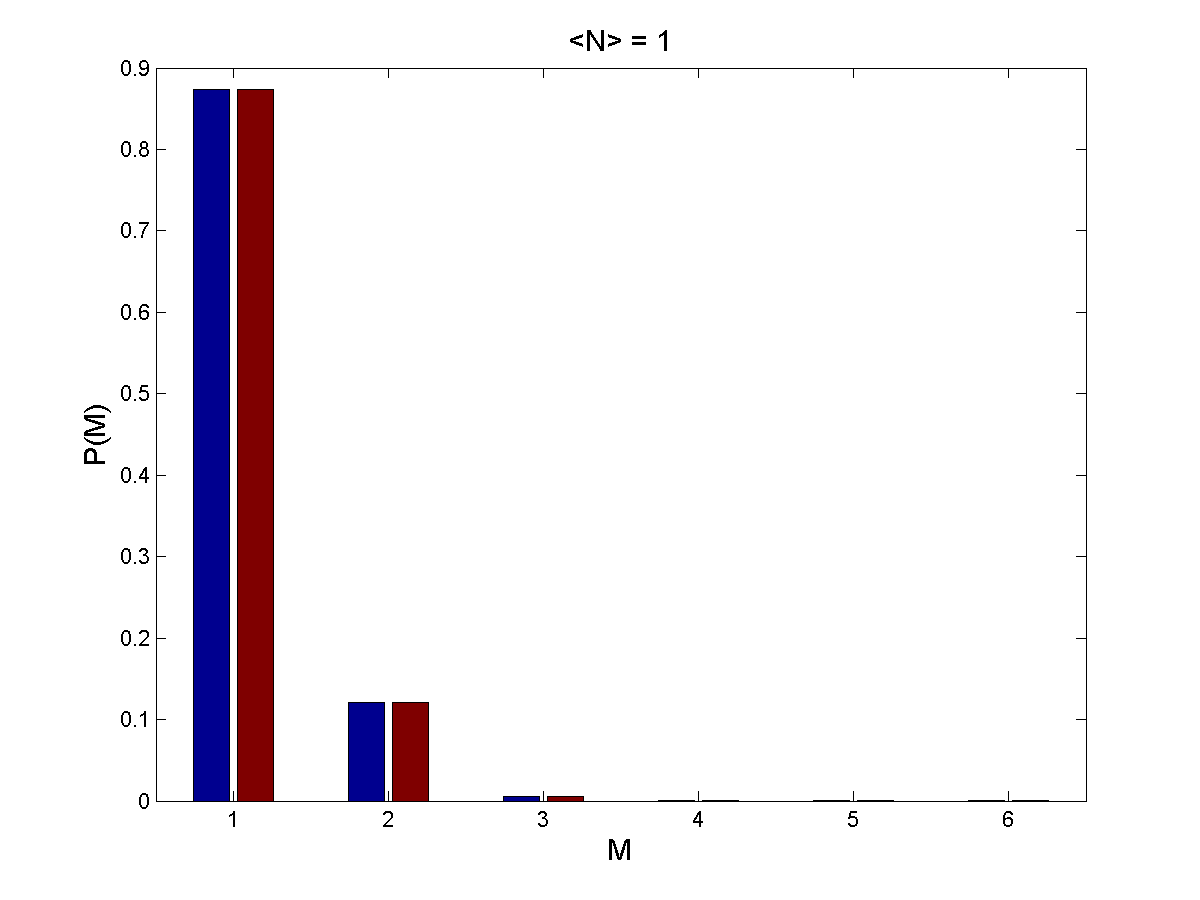
\includegraphics[width=14cm]{slike/plot2}
\caption{Verjetnost dolžine niza $P_+(M)$ v odvisnosti od njegove dolžine $M$, $\bar{N}=1$}
\label{plot2}
\end{center}
\end{figure}

\section{Numerični račun}

\subsection{"Run-up" test}

Za preizkus generatorjev naključnih števil uporabimo "run-up" test: v danem vzorcu številu preštejemo striktno naraščujoče nize z dolžino M in jih primerno normaliziramo, da dobimo delež teh nizov $P'$.
\[
P_+' = \frac{N_+}{N_+ + N_- + N_=}
\]
\[
P'(M) = \frac{N(M)}{ \sum_{m=1}^{\inf} N(m)}
\]
\[
P_+'(M) = P'(+) \cdot P'(M) = \frac{N_+ N(M)}{(N_+ + N_- + N_=) \cdot \sum_{m=1}^{\inf}N(m)}
\]

Delež strogo naraščujočih nizov še normaliziramo, da je primerljiv z izračunano verjetnostjo: $\sum_{m=1}^{\inf} P_+'(m) = 1$.

\subsection{Generatorji}

Za analizo uporabimo sete števil dolžine $10^6$ iz različnih virov, porazdeljenih po naključni poissonovi porazdelitvi z $\bar{N}=1$. Večina generatorjev te porazdelitve uporablja algoritem opisan v \cite[str.~504]{devroye}, ki iz uniformne porazdelitve generira poissonovo.\\
Uporabimo generatorje iz različnih okolij: numpy.random.poisson, Octave/Matlab - poissrnd, Octave/Matlab - rand + Devroye, R - rpois, PHP rand@Windows + Devroye.

S spletne strani random.org je mogoče dobiti tudi prave (tako trdi avtor) naključne podatke, vendar v omejenih količinah - uporabili smo niz $10^3$ uniformno porazdeljenih števil iz intervala [0,1).

Rezultate prikažemo na sliki \ref{plot5} in približane na sliki \ref{plot6}:

\begin{figure}[H]
\begin{center}
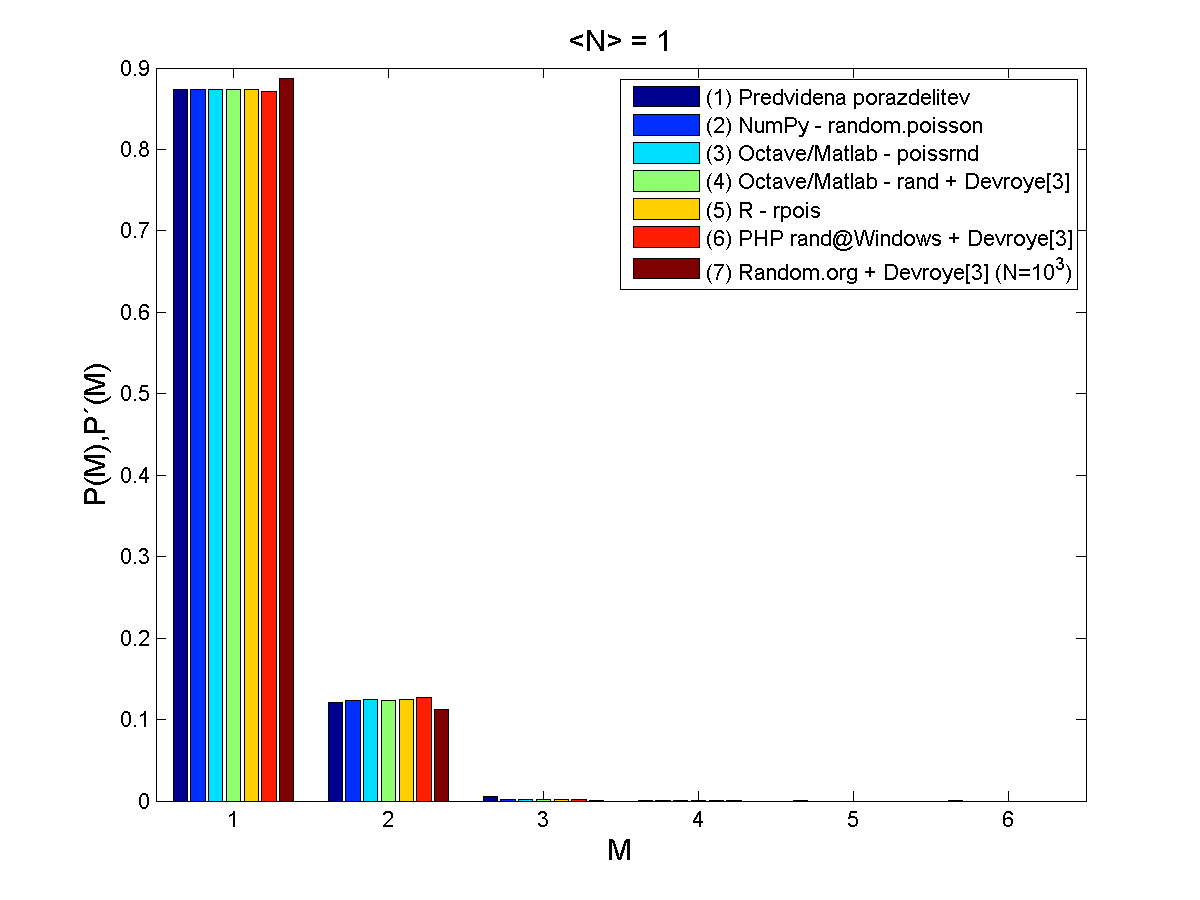
\includegraphics[width=14cm]{slike/plot5}
\caption{Normaliziran delež naraščujočih nizov ($P_+'(M)$) in verjetnost za dolžino naraščujočih nizov ($P_+(M)$) v odvisnosti od njihove dolžine $M$. $\bar{N}=1$}
\label{plot5}
\end{center}
\end{figure}

\newpage

\section{Zaključek}
Izkaže se da je računanje verjetnosti za daljše strogo naraščujoče nize v poissonovi porazdelitvi računsko zahtevna naloga, vendar imajo pri previdno izbranem $\bar{N}$ kratek rep, kar nalogo precej olajša.

Po grafih sklepamo, da večina priljubljenih računskih paketov generira zelo dobre nize poissonovih naključnih števil, saj so razlike med deleži v generiranih nizih, deleži v nizu naključnih števil in pričakovanimi verjetnostmi dolžin velikostnega reda $10^3$.

\begin{figure}[H]
\begin{center}
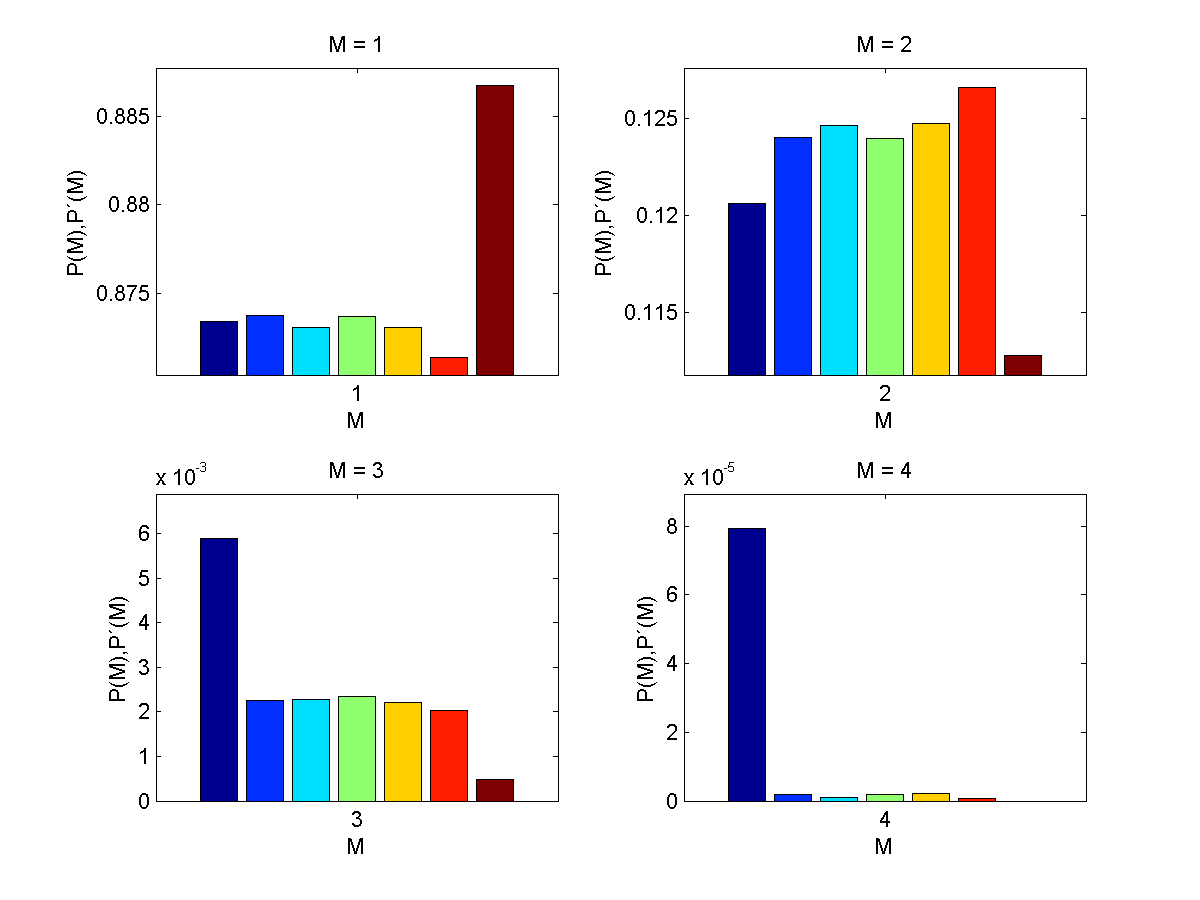
\includegraphics[width=13cm]{slike/plot6}
\caption{Normaliziran delež naraščujočih nizov ($P_+'(M)$) in verjetnost za dolžino naraščujočih nizov ($P_+(M)$) v odvisnosti od njihove dolžine $M$. $\bar{N}=1$}
\label{plot6}
\end{center}
\end{figure}

\begin{thebibliography}{99}

\bibitem{kodre} I. Kuščer in A. Kodre: Matematika v fiziki in tehniki, DMFA, Ljubljana, 1994
\bibitem{matlabDoc} Dokumentacija programa Matlab - http://www.mathworks.com/help/techdoc/
\bibitem{devroye} Luc Devroye: Non-uniform random variate generation, Springer-Verlag New York, 1986 (http://www.eirene.de/Devroye.pdf)

%  I. Priimek, Naslov knjige, Zalo?nik, MestoIzdaje, Letnica.
% \bibitem{oznakaClanka} I. Priimek, Naslov ?lanka, Naslov revije Letnik (Leto) str.\ Od--Do.
\end{thebibliography}


% \subsection{Prvi podrazdelek prvega razdelka}

% Tu napišete vsebino prvega podrazdelka prvega razdelka. \LaTeX je namenjen predvsem matematičnim besedilom. Vsaka matematična formula, tudi zgolj $x$, se pojavi med dvema \$ znakoma: \verb.$x$.. Seveda pa lahko napišemo tudi bolj zapletene izraze: $$\int_0^\infty \frac{1}{x^3}dx.$$


% \begin{izrek}
% \label{iz:prviIzrek}
% Tu napišete besedilo izreka.
% \end{izrek}
% \begin{dokaz}
% Tu napišete besedilo dokaza. Lahko je dolgo več vrstic, ali pa sem in tja % preide tudi v nov odstavek.

%Nov odstavek se začne po prazni vrstici.
%\end{dokaz}


% Sledi še primer naštevanja z možnim sklicevanjem, npr. na Izrek \ref{iz:prviIzrek}: 
% \begin{enumerate}[label=(\roman{*}), ref=(\roman{*})]
% \item \label{it:prva} Prva alineja je pred alinejo \ref{it:druga}.
% \item \label{it:druga} Druga alineja sledi alineji \ref{it:prva}.
% \end{enumerate}


\end{document}
